% Chapter 8
\section[Nonlinear latent spaces and kernels]{Nonlinear Latent Spaces: Linear Regression as a Natural Kernel Method}\label{sec:kernel}

Chapter~\ref{sec:intro} said it: ``linear'' is a requirement on the \textbf{parameters}, not on the raw variables. This chapter pushes that sentence to its limit. Suppose the observed features are in fact nonlinear projections of high-dimensional latent variables
\begin{equation}\label{eq:feature-map}
  \x_i = \phi(\bm{z}_i), \qquad \bm{z}_i \in \R^q \ \text{(latent)}, \quad \phi : \R^q \to \R^d \ \text{(feature map)},
\end{equation}
where the dimension $d$ may be arbitrarily large --- including infinite. Running least squares on $\y = \X \bbeta + \bm{\varepsilon}$ is then simply pointing the entire machinery of Chapters~\ref{sec:highdim}--\ref{sec:gd-underdet} at the feature matrix
\[
  \bm{\Phi} := \big[\phi(\bm{z}_1)^\top;\ \dots;\ \phi(\bm{z}_n)^\top\big] \in \R^{n \times d} .
\]
The core conclusion of this chapter: \textbf{the linear regression between $\X$ and $\y$ behaves, in the world of the latent variables $\bm{z}$, as a kernel method --- the prediction is nonlinear in $\bm{z}$, yet the computation only needs the $n \times n$ kernel matrix}.

\subsection{Kernels and Gram matrices: the inner product as the only interface}\label{sec:kernel-def}

Define the \textbf{kernel function} as the inner product in feature space
\begin{equation}\label{eq:kernel}
  k(\bm{z}, \bm{z}') = \big\langle \phi(\bm{z}),\ \phi(\bm{z}') \big\rangle ,
\end{equation}
together with the sample Gram matrix and the kernel vector of a new point
\begin{equation}\label{eq:gram}
  \bm{K} = \bm{\Phi} \bm{\Phi}^\top \in \R^{n \times n},
  \qquad
  K_{ij} = k(\bm{z}_i, \bm{z}_j);
  \qquad
  \bm{k}(\bm{z}) = \bm{\Phi}\, \phi(\bm{z}) = \big( k(\bm{z}, \bm{z}_1), \dots, k(\bm{z}, \bm{z}_n) \big)^\top .
\end{equation}
Note that \textbf{no coordinate of $\phi$ appears in \eqref{eq:gram}} --- the whole idea of kernel methods is: if every intermediate quantity of an algorithm can be written in terms of inner products $\langle \phi(\cdot), \phi(\cdot)\rangle$, then $\phi$ never needs to be constructed explicitly, and $d = \infty$ is just as fine. Mercer's theorem guarantees that every positive-definite kernel $k$ corresponds to some (possibly infinite-dimensional) feature map $\phi$; the two are two faces of the same object\cite{scholkopf2002}.

\subsection[$d > n$: kernel form of the underdetermined closed form]{$d > n$: the kernel form of $\widehat{\bbeta}'$}\label{sec:kernel-underdet}

Substitute $\bm{\Phi}$ for $\X$ in the underdetermined closed form $\widehat{\bbeta}' = \X^\top(\X\X^\top)^{-1}\y$ of Chapter~\ref{sec:gd-underdet}. For a new sample $\tilde{\x} = \phi(\tilde{\bm{z}})$, the prediction is
\begin{equation}\label{eq:kernel-interp}
  \tilde{\x}^\top \widehat{\bbeta}'
  = \phi(\tilde{\bm{z}})^\top \bm{\Phi}^\top (\bm{\Phi}\bm{\Phi}^\top)^{-1} \y
  = \bm{k}(\tilde{\bm{z}})^\top \bm{K}^{-1} \y .
\end{equation}
Check every object in this line step by step: $\bm{\Phi}\bm{\Phi}^\top = \bm{K}$ is the kernel matrix; $\phi(\tilde{\bm{z}})^\top \bm{\Phi}^\top = \bm{k}(\tilde{\bm{z}})^\top$ is the kernel vector. \textbf{The prediction is written entirely in terms of the kernel function.} Written as an expansion,
\begin{equation}\label{eq:kernel-expansion}
  \hat{f}(\tilde{\bm{z}}) = \tilde{\x}^\top \widehat{\bbeta}' = \sum_{i=1}^n \alpha_i\, k(\tilde{\bm{z}}, \bm{z}_i),
  \qquad
  \bm{\alpha} = \bm{K}^{-1} \y ,
\end{equation}
i.e., the prediction is a \textbf{linear combination of kernel sections anchored at the training points} --- this is \textbf{kernel interpolation}, also known as kernel ridgeless regression: it is the minimum-norm interpolating solution in $d > n$ feature space (Section~\ref{sec:minnorm}) expressed in kernel language, and for a positive-definite kernel the feature-space norm is exactly the RKHS norm --- \textbf{the point GD converges to from zero is simultaneously the interpolating function of minimal norm in the RKHS}\cite{kimeldorf1970}. This is the kernel form of the $(\phi(\bm{Z})\phi(\bm{Z})^\top)^{-1}$ in the original question: \textit{it never needs to be constructed --- it is simply $\bm{K}^{-1}$, assembled directly from kernel values}.

\subsection[Kernel form of the OLS closed form and the push-through identity]{$n \gg d$: the kernel form of $\bhat$ and the push-through identity}\label{sec:kernel-overdet}

Substitute $\bm{\Phi}$ for $\X$ in the closed form $\bhat = (\X^\top\X)^{-1}\X^\top\y$ of Section~\ref{sec:hd-closed}; the prediction becomes $\phi(\tilde{\bm{z}})^\top (\bm{\Phi}^\top\bm{\Phi})^{-1} \bm{\Phi}^\top \y$. Trouble: the entries of $\bm{\Phi}^\top\bm{\Phi} \in \R^{d \times d}$ are $\sum_i \phi_a(\bm{z}_i)\phi_b(\bm{z}_i)$ --- \textbf{cross terms of feature coordinates, not determined by the kernel matrix $\bm{K}$ alone}. This is exactly the dividing line of ``when kernelization is possible'': quantities that depend only on pairwise inner products of the observed points can be kernelized; quantities that depend on the feature coordinate system itself cannot.

The way out is the ridge regularization already familiar from Section~\ref{sec:hd-break} --- it both repairs ill-conditioning and, as it happens, completes the kernelization. With $\lambda$ added, the prediction is $\phi(\tilde{\bm{z}})^\top(\bm{\Phi}^\top\bm{\Phi} + \lambda \bm{I}_d)^{-1}\bm{\Phi}^\top\y$, and the \textbf{push-through identity} (verify by multiplying both sides on the left by $(\bm{\Phi}^\top\bm{\Phi} + \lambda\bm{I})$)
\begin{equation}\label{eq:push-through}
  (\bm{\Phi}^\top\bm{\Phi} + \lambda \bm{I}_d)^{-1} \bm{\Phi}^\top
  = \bm{\Phi}^\top (\bm{\Phi}\bm{\Phi}^\top + \lambda \bm{I}_n)^{-1}
  = \bm{\Phi}^\top (\bm{K} + \lambda \bm{I}_n)^{-1},
\end{equation}
has only kernel objects on the right-hand side. Hence \textbf{kernel ridge regression}
\begin{equation}\label{eq:kernel-ridge}
  \hat{f}(\tilde{\bm{z}}) = \bm{k}(\tilde{\bm{z}})^\top (\bm{K} + \lambda \bm{I}_n)^{-1} \y .
\end{equation}
This is the kernel form of the $(\phi(\bm{Z})^\top\phi(\bm{Z}))^{-1}$ from the original question: \textit{it is first regularized by $\lambda$, then flipped through the sample space by push-through, becoming $(\bm{K} + \lambda\bm{I}_n)^{-1}$ --- the $d \times d$ inverse in the original space is never computed}. Letting $\lambda \to 0^+$, \eqref{eq:kernel-ridge} formally recovers \eqref{eq:kernel-interp}: \textbf{the two regimes converge in kernel language}. Gaussian process regression is the Bayesian retelling of the same object (kernel = covariance function, posterior mean = \eqref{eq:kernel-ridge})\cite{scholkopf2002}.

\subsection{Examples: when a kernel is ``natural''}\label{sec:kernel-examples}

\begin{itemize}
  \item \textbf{Polynomial kernel} $k(\bm{z}, \bm{z}') = (\bm{z}^\top \bm{z}' + c)^m$: corresponds to an explicit finite-dimensional feature map (all monomials of degree $\le m$), with $d = \binom{q+m}{m}$ --- a finite-dimensional regression with $n \gg d$, where kernelization is merely a convenience.
  \item \textbf{Gaussian kernel} (RBF) $k(\bm{z}, \bm{z}') = \exp\!\big( -\norm{\bm{z} - \bm{z}'}^2 / 2\sigma^2 \big)$: the corresponding $\phi$ is \textbf{infinite-dimensional} and cannot be constructed explicitly --- here kernelization is not a trick but the \textit{only} way out. The $d > n$ story of \eqref{eq:kernel-interp} naturally lives here.
  \item \textbf{Random features} (Rahimi \& Recht, 2007): going the other direction, approximate the Gaussian kernel back to a \textbf{finite} dimension via $\phi(\bm{z}) = \sqrt{\tfrac{2}{D}}\big(\cos(\bm{\omega}_1^\top \bm{z} + b_1), \dots\big)$ (random frequencies) and then run all the $d$-dimensional linear algebra of this chapter --- as $d \to \infty$, random-feature regression converges to kernel regression\cite{rahimi2007}. This route welds ``kernel methods'' and ``wide neural networks'' together: random-feature regression is precisely the linear version of the function-space limit of a two-layer infinitely wide network.
\end{itemize}

\begin{figure}[htbp]
  \centering
  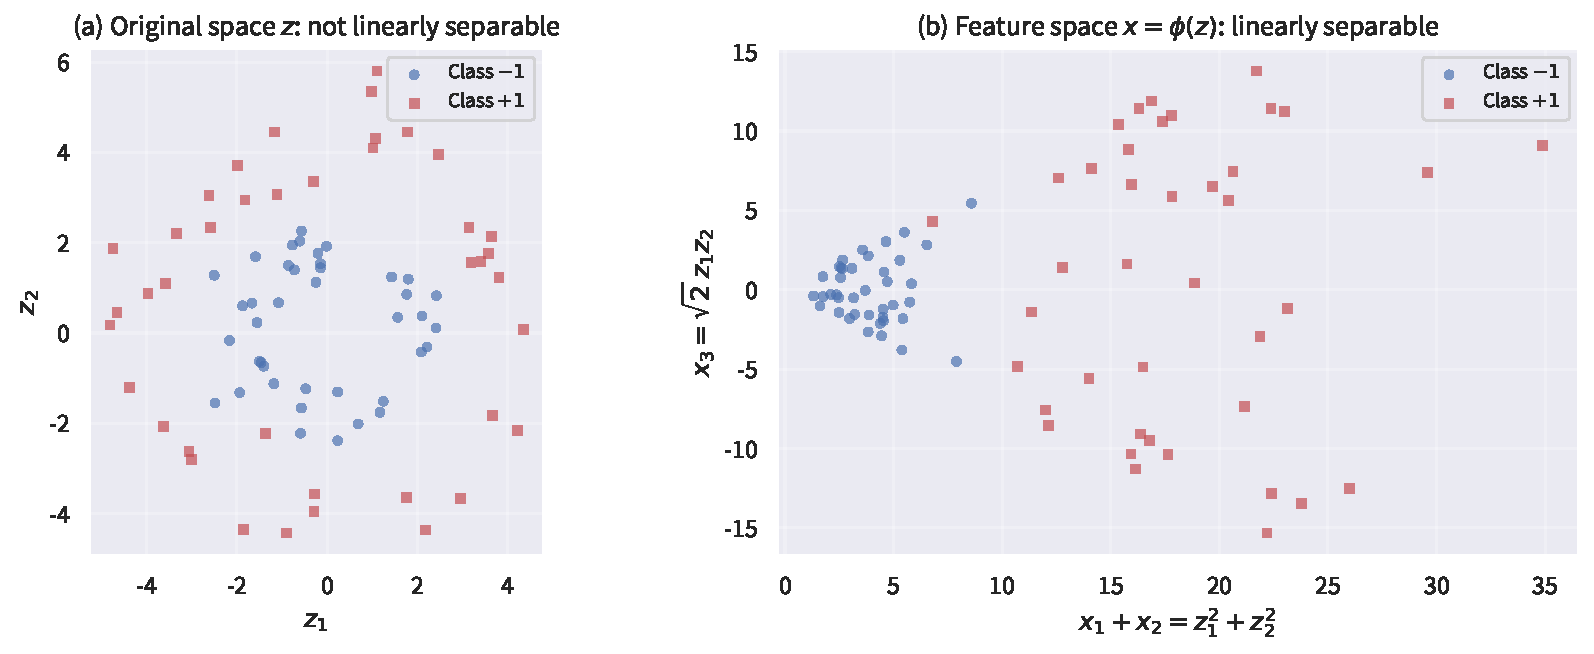
\includegraphics[width=\linewidth]{figures/ch7_kernel.pdf}
  \caption{The geometric essence of kernel methods: the same ring-shaped data (two classes by radius) cannot be separated by any straight line in the original latent space $z$ (left); lifted by the quadratic feature map $\phi(z)=(z_1^2, z_2^2, \sqrt{2}z_1z_2)$ into feature space (right), a single linear function separates them. \textbf{Linear in $x$ $=$ nonlinear in $z$} --- and hence the prediction of linear regression becomes a natural nonlinear method in latent space.}
  \label{fig:ch7-kernel}
\end{figure}

\subsection[From kernel regression to deep networks: ridgeless regression, Fourier features, and the NTK]{From kernel regression to deep networks: ridgeless regression, Fourier features, and the neural tangent kernel}\label{sec:ntk}

This chapter closes by doing something that ``collects the whole book'': walking the road ``linear regression $\to$ kernel regression'' all the way to the doorstep of \textbf{deep neural networks}. There are two bridges along the way: the first is \textbf{random Fourier features} (the old bridge, 2007), the second is the \textbf{neural tangent kernel} (NTK, the new bridge, 2018)\cite{jacot2018}.

\subsubsection*{Bridge one: a two-layer network = linear regression on random features}

Consider the simplest two-layer network
\begin{equation}\label{eq:two-layer}
  f(\bm{z}; \bm{a}) = \frac{1}{\sqrt{D}} \sum_{j=1}^{D} a_j\, \sigma\big( \bm{\omega}_j^\top \bm{z} + b_j \big),
\end{equation}
where $\sigma$ is an activation (ReLU, tanh, \dots), the first-layer parameters $(\bm{\omega}_j, b_j)$ are \textbf{randomly sampled from some distribution and then frozen}, and only the second layer $\bm{a} \in \R^D$ is trained. Note two things:

\begin{enumerate}[label=(\arabic*)]
  \item With $\phi(\bm{z}) = \tfrac{1}{\sqrt{D}}\big(\sigma(\bm{\omega}_1^\top\bm{z}+b_1), \dots, \sigma(\bm{\omega}_D^\top\bm{z}+b_D)\big)^\top$, we have $f(\bm{z};\bm{a}) = \phi(\bm{z})^\top\bm{a}$ --- \textbf{it is simply linear regression in $\bm{a}$}, and the entire machinery of this chapter (normal equations, exact GD solution, push-through, the kernelization criterion) applies verbatim.
  \item If $\bm{a}$ is initialized at zero and trained by gradient descent, the implicit-regularization analysis of Chapter~\ref{sec:implicit} says: it converges to the \textbf{minimum-norm} interpolating solution --- in the Euclidean norm of $\bm{a}$. This is \textbf{ridgeless regression} (ridge with $\lambda \to 0^+$, see Exercise~\ref{ex:ridge-dual}): \textit{with no explicit penalty at all, the interpolating solution of smallest norm is automatically selected by GD}.
\end{enumerate}

By \eqref{eq:kernel-interp}, its prediction takes the same kernel form, only with the kernel replaced by the \textbf{random-feature kernel}
\begin{equation}\label{eq:rf-kernel}
  k_{\mathrm{RF}}(\bm{z}, \bm{z}') = \frac{1}{D}\sum_{j=1}^D \sigma(\bm{\omega}_j^\top\bm{z}+b_j)\,\sigma(\bm{\omega}_j^\top\bm{z}'+b_j)
  \ \xrightarrow{D \to \infty}\ \E_{\bm{\omega}, b}\big[ \sigma(\bm{\omega}^\top\bm{z} + b)\,\sigma(\bm{\omega}^\top\bm{z}' + b) \big],
\end{equation}
which is exactly the theoretical core of Rahimi \& Recht's random Fourier features (for shift-invariant kernels, taking $\sigma = \cos$ with a specific sampling distribution makes \eqref{eq:rf-kernel} reproduce the Gaussian kernel exactly)\cite{rahimi2007}. \textbf{One sentence: freeze the first layer, train the second, initialize at zero, run gradient descent $=$ ridgeless regression in a Fourier-feature space.}

\subsubsection*{Bridge two: the NTK --- with all parameters trained, function space stays linear}

Bridge one leaves an ``unnatural'' assumption: the first layer is frozen. What if \textbf{all} parameters $\bm{\theta} = (\bm{a}, \{ \bm{\omega}_j, b_j \})$ are trained? The loss in parameter space,
\[
  L(\bm{\theta}) = \frac{1}{2}\sum_{i=1}^n \big( f(\bm{z}_i; \bm{\theta}) - y_i \big)^2,
\]
is in general \textbf{nonconvex} --- the source of deep learning's ``mystery.'' The key observation of Jacot, Gabriel, and Hongler is: stop staring at parameter space; stare at \textbf{function space}. For the residual vector $\bm{r}_t = \big( f(\bm{z}_i; \bm{\theta}_t) - y_i \big)_i$ on the training set, the chain rule gives
\begin{equation}\label{eq:ntk-flow}
  \frac{d\, f(\bm{z}; \bm{\theta}_t)}{dt}
  = \nabla_{\bm{\theta}} f(\bm{z}; \bm{\theta}_t)^\top \frac{d\bm{\theta}_t}{dt}
  = -\sum_{i=1}^n \underbrace{\big\langle \nabla_{\bm{\theta}} f(\bm{z}; \bm{\theta}_t),\ \nabla_{\bm{\theta}} f(\bm{z}_i; \bm{\theta}_t) \big\rangle}_{\Theta_t(\bm{z}, \bm{z}_i)} \, r_{t,i} ,
\end{equation}
where
\begin{equation}\label{eq:ntk-def}
  \Theta_t(\bm{z}, \bm{z}') := \big\langle \nabla_{\bm{\theta}} f(\bm{z}; \bm{\theta}_t),\ \nabla_{\bm{\theta}} f(\bm{z}'; \bm{\theta}_t) \big\rangle
\end{equation}
is the \textbf{neural tangent kernel}. The shape of \eqref{eq:ntk-flow} should look familiar: it is \textbf{kernel gradient descent in function space} --- isomorphic to $\widehat{\bbeta}_{t+1} = \widehat{\bbeta}_t - \eta\,\X^\top(\X\widehat{\bbeta}_t - \y)$ of Chapter~\ref{sec:gd}, except that ``inner products of the design matrix'' are replaced by ``inner products of parameter gradients.''

The astonishing fact about the NTK is its \textbf{wide-network limit}: with $\tfrac{1}{\sqrt{D}}$ scaling (as in \eqref{eq:two-layer}), as the width $D \to \infty$:

\begin{enumerate}[label=(\arabic*)]
  \item at initialization, $\Theta_0$ converges by the law of large numbers to a \textbf{deterministic kernel} $\Theta$ (for two-layer networks it can be computed explicitly; see Exercise~\ref{ex:ntk});
  \item throughout \textbf{the entire training}, $\Theta_t$ stays put ($\Theta_t \to \Theta$, with no drift in $\bm{\theta}_t$) --- parameters travel far, the kernel never moves;
  \item hence \eqref{eq:ntk-flow} becomes a \textbf{linear} ODE $\frac{df_t(\bm{z})}{dt} = -\sum_i \Theta(\bm{z},\bm{z}_i)\, r_{t,i}$, whose solution converges exponentially along the eigendirections of $\Theta$, with limit
  \begin{equation}\label{eq:ntk-ridgeless}
    f_\infty(\tilde{\bm{z}}) = \bm{\Theta}(\tilde{\bm{z}})^\top \bm{\Theta}^{-1} \y,
  \end{equation}
  where $\bm{\Theta} = \big(\Theta(\bm{z}_i,\bm{z}_j)\big)_{ij}$ is the Gram matrix of the NTK at the training points and $\bm{\Theta}(\tilde{\bm{z}})$ is the kernel vector of the new sample.
\end{enumerate}

Equation \eqref{eq:ntk-ridgeless} is \textbf{isomorphic to \eqref{eq:kernel-interp} symbol by symbol}: the function-space limit, under gradient descent, of an infinitely wide two-layer (indeed arbitrarily deep\cite{lee2019}) neural network with all parameters trained, is exactly \textbf{ridgeless kernel regression with the NTK as kernel}. The nonconvexity of parameter space is an ``illusion of the coordinate system'' --- switch to function space, and deep-network training is Chapter~5's minimum-norm interpolation story all over again.

\begin{keybox}[The bridge from a straight line to deep networks]
\[
\resizebox{0.97\textwidth}{!}{$\begin{gathered}
\text{linear regression } \xrightarrow{\ \phi\ } \text{ kernel regression } \xrightarrow[\text{made explicit}]{\ \text{random Fourier features}\ } \text{ finite-dimensional ridgeless regression} \\
\xrightarrow[\text{all parameters trained, wide limit}]{\ \mathrm{NTK}\ } \text{ the function-space limit of deep networks}
\end{gathered}$}
\]
The four arrows are supported, respectively, by Section~\ref{sec:kernel-overdet} (push-through), \eqref{eq:rf-kernel} (the law of large numbers), Chapter~\ref{sec:implicit} (implicit regularization), and \eqref{eq:ntk-ridgeless} (NTK constancy). \textbf{Linear regression is not a special case of deep learning; the wide limit of deep learning is the kernelization of linear regression} --- which is why a two-hundred-year-old straight line remains the most honest starting point for understanding every model today.
\end{keybox}

Two pragmatic remarks. First, the NTK describes the \textit{lazy training} regime: large parameter-initialization scale, small training displacement --- the network is ``too lazy'' to change its internal features. When feature learning actually happens in real deep learning, the NTK fails, and theory is still under construction (Jacot's own subsequent work distinguishing the lazy regime from the feature-learning regime is exactly about this). Second, ridgeless interpolation is \textbf{not only harmless --- it can be better}: Belkin et al.'s double-descent observation shows that the test error of modern overparameterized models keeps decreasing past the interpolation threshold\cite{belkin2019} --- the minimum-norm solution of Chapter~\ref{sec:minnorm} is the cleanest linear incarnation of this phenomenon, and work of Jingfeng Wu et al.\ further shows that optimally early-stopped GD statistically dominates optimally tuned ridge (see the preface and the bibliography)\cite{wu2025}. Put these two remarks next to \eqref{eq:ntk-ridgeless}, and you hold the most honest linear answer currently available to ``why do overparameterized networks generalize?''

\begin{figure}[htbp]
  \centering
  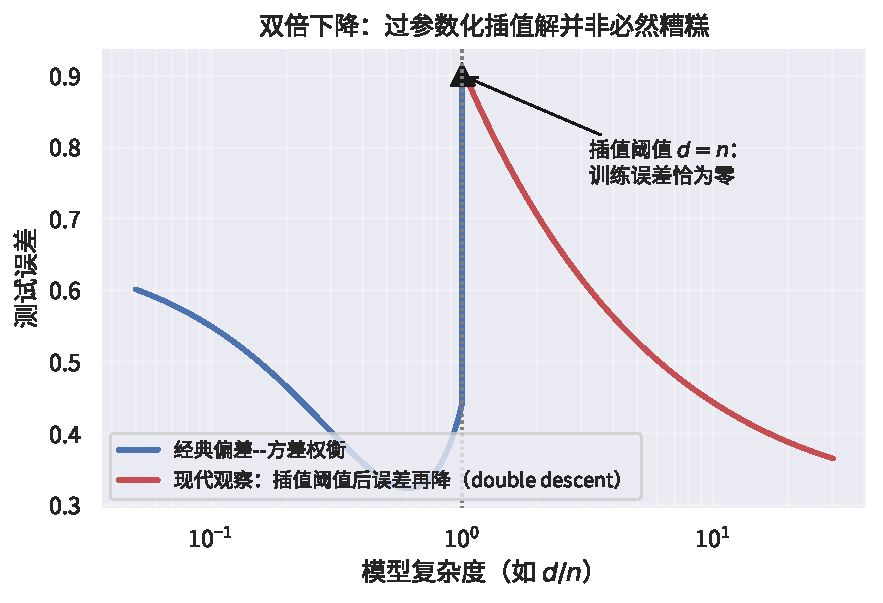
\includegraphics[width=0.72\linewidth]{figures/ch7_doubledescent.pdf}
  \caption{Double descent (schematic; Belkin et al., 2019\cite{belkin2019}): classical textbooks say test error is optimal near $d \approx n$ (blue, U-shape); modern observation shows the error spikes at the interpolation threshold $d=n$ and then \textbf{keeps decreasing} (red) --- interpolation itself is no sin; what matters is \emph{which} interpolating solution implicit regularization selects. Ridgeless regression and early-stopped GD give the linear account of this selection.}
  \label{fig:ch7-doubledescent}
\end{figure}

\begin{exercise}\label{ex:ntk}
For the two-layer network \eqref{eq:two-layer} (smooth $\sigma$), let $(\bm{\omega}_j, b_j) \sim \mathcal{N}(\zero, \bm{I})$ i.i.d.\ and $\bm{a}$ be initialized independently with $\E[a_j^2] = 1$. Verify: as $D \to \infty$, the NTK at initialization \eqref{eq:ntk-def} converges pointwise to
\[
  \Theta(\bm{z},\bm{z}') = \E\big[ \sigma(\bm{\omega}^\top\bm{z}+b)\,\sigma(\bm{\omega}^\top\bm{z}'+b) \big] \;+\; \bm{z}^\top\bm{z}'\, \E\big[ \sigma'(\bm{\omega}^\top\bm{z}+b)\,\sigma'(\bm{\omega}^\top\bm{z}'+b) \big],
\]
and identify which term comes from the gradients of the last-layer parameters and which from the first-layer parameters; then explain why the second term (absent from the random-feature kernel \eqref{eq:rf-kernel}) makes the NTK strictly stronger than the random-feature kernel. For $\sigma = \mathrm{ReLU}$, use the half-space moment formulas of the Gaussian distribution to write both expectations explicitly in terms of the angle between $\bm{z}$ and $\bm{z}'$.
\end{exercise}

\subsection{Conclusion of this chapter}\label{sec:kernel-conclusion}

\begin{keybox}[Takeaways]
\begin{itemize}
  \item With $\x_i = \phi(\bm{z}_i)$, writing $\bm{K}_{ij} = k(\bm{z}_i,\bm{z}_j)$ and $\bm{k}(\tilde{\bm{z}})_i = k(\tilde{\bm{z}}, \bm{z}_i)$, we have
  \[
    d > n:\ \tilde{\x}^\top \widehat{\bbeta}' = \bm{k}(\tilde{\bm{z}})^\top \bm{K}^{-1} \y
    \ \xrightarrow{\ \lambda\ }\ 
    n \gg d:\ \tilde{\x}^\top \bhat^{\mathrm{ridge}} = \bm{k}(\tilde{\bm{z}})^\top (\bm{K} + \lambda \bm{I})^{-1} \y .
  \]
  Both closed-form solutions of linear regression are \textbf{estimators assembled purely from the kernel function};
  \item The two key steps of kernelization: inner-product-ization (write every quantity as $\langle\phi,\phi\rangle$) and push-through ($(\bm{\Phi}^\top\bm{\Phi} + \lambda\bm{I})^{-1}\bm{\Phi}^\top = \bm{\Phi}^\top(\bm{K} + \lambda\bm{I})^{-1}$) --- the latter flips the inverse from feature space into sample space;
  \item The prediction $\hat{f}(\tilde{\bm{z}}) = \sum_i \alpha_i k(\tilde{\bm{z}}, \bm{z}_i)$ is \textbf{nonlinear} in the latent variables $\bm{z}$, even though it is linear in $\x = \phi(\bm{z})$ --- ``the prediction of linear regression is a natural kernel method under nonlinear latent-space mappings'' is now proved;
  \item At $d = \infty$ (Gaussian kernel) kernelization goes from convenience to necessity; random features go the other way and approximate the kernel back into finite-dimensional linear algebra, welding the route back to parameterized networks.
\end{itemize}
\end{keybox}

\begin{exercise}\label{ex:kernel-dual}
Use \eqref{eq:push-through} to prove that the primal and dual forms of kernel ridge regression give \textbf{exactly the same} prediction function, and explain why no rank assumption is needed when $\lambda > 0$.
\end{exercise}

\begin{exercise}\label{ex:kernel-interp}
Verify that the Gaussian kernel matrix $\bm{K}$ (with distinct samples) is positive definite and invertible, so that \eqref{eq:kernel-interp} is well defined; further verify that $\bm{\alpha}$ in \eqref{eq:kernel-expansion} satisfies $\bm{K}\bm{\alpha} = \y$ (the kernel interpolation equation), and connect it with the interpolation verification \eqref{eq:interp} of Chapter~\ref{sec:gd-underdet}.
\end{exercise}
